\documentclass[a4paper,10pt]{article}
%
\usepackage{amsmath}
\usepackage{amssymb}
\usepackage{amstext}
\usepackage[bookmarks,colorlinks]{hyperref}
\usepackage{makeidx}
\usepackage{graphicx}
\usepackage{longtable}
\usepackage{multirow}
\usepackage{listings}
\usepackage{xcolor}
\usepackage{float}
\usepackage{booktabs}

\makeindex

\usepackage{geometry}
\geometry{left=3cm,right=4cm,top=4cm,bottom=4cm}

\lstset{numbers=left, numberstyle=\tiny, basicstyle=\tiny, keywordstyle=\color{blue!70}, commentstyle=\color{red!50!green!50!blue!50}, frame=shadowbox, rulesepcolor=\color{red!20!green!20!blue!20},escapeinside=``, xleftmargin=2em,xrightmargin=2em, aboveskip=1em}

\begin{document}
%-----------------------------------------------------------

\title{Design of HugeDB, Draft}
\author{Wei Cao}
\maketitle

\begin{abstract}
The SequentialDB data structure is not suitable for large number of random insertions, however many applications rely on such kind of behavior, for example, SDBTrie and offline algorithms in MIA.
Experiment result and a further analysis show, the problem of SequentialDB can be due to inefficient random disk reads and writes during random insertion.
So the HugeDB is proposed to replace SequentialDB in such kind of environment. Two major techniques have been raised here to eliminate both random disk reads and random disk writes.
One is merge-based incremental growth, which may cause find operations slow down a little if db partitions are unmerged.
The other is modification tag method, at the cost of adding a meta field in each record to store modification type.
However, the price worth the gain on IO in applications mentioned above.
\end{abstract}

%--------------------------------------------------
\tableofcontents
%--------------------------------------------------

\section{Document History}
\begin{center}
\begin{tabular}{|c|c|p{7cm}|}
    \hline
    Date & Author & Description \\ \hline
    2009-09-16& Wei Cao & An inital version for explaining and reviewing the overall design. \\ \hline
\end{tabular}
\end{center}

\section{Introduction}
From now on, for simplity, \emph{sdb} always stands for SequentialDB, while \emph{hdb} is short for HugeDB.

There are two types of sdb, sdb\_hash and sdb\_btree, keys in sdb\_hash are unordered while has order in sdb\_btree, so an advantage of btree over hash is btree could be used for range search.
The items in a range of $[x,y]$ can be found by searching for x in the tree, then performing an inorder traversal in the tree from x to y.
Although both suffers from rapid performance degradation when db gets large, I focus on sdb\_btree, since it's worse and more representive.
Following table shows, given plenty of memory (1G), how insertion time increase, they are measured between inserting every 1,000,000 $<int, int>$ records into a sdb\_btree continously.

\begin{table}[H]\centering
\begin{tabular}[t]{c|p{8cm}}
     \toprule
     Number of records in sdb\_btree & Time spent on inserting next 1,000,000 records\\
     \midrule
     $\leq$ 21,000,000 & $\leq$ 1.25 second \\
     \textbf{22,000,000} & \textbf{19.9 seconds} \\
     23,000,000 & 20.2 seconds \\
     ...        & ...  \\
     32,000,000 & 39.0 seconds\\
     33,000,000 & 41.4 seconds\\
     34,000,000 & 42.4 seconds\\
     35,000,000 & 58.5 seconds\\
     36,000,000 & 1.7 minute \\
     37,000,000 & 3.3 minutes \\
     38,000,000 & 3.4 minutes \\
     39,000,000 & 3.6 minutes \\
     40,000,000 & 4.1 minutes \\
     41,000,000 & 4.3 minutes \\
     42,000,000 & 4.8 minutes \\
     \textbf{43,000,000} & \textbf{16.3 minute}s \\
     44,000,000 & 17.1 minutes \\
     \bottomrule
\end{tabular}
\end{table}

There are two sharp points in the table:
\begin{enumerate}
\item The first point is at 22,000,000, before that, all records are kept in memory cache, so insertion speed is rather fast, less than 1.25 second.
But at the point, memory cache becomes full, sdb\_btree begins continously flushing dirty nodes to disk and loading newly accessed nodes into memory, insertion speed decreases to 19.9 seconds immediately.
\item The second point is at 43,000,000, sdb file's size increase to 2.4G at this point, occupying nearly all 2G physical memory on my machine. The operating system cannot cache the whole file in memory any more,
so the OS begins swapping file pages between memory and disk after that point, which causes insertion speed slows down for 4 times immediately.
\end{enumerate}
Above experiment shows, speed of random insertions in sdb\_btree degrades too rapidly. Imagine, 22,000,000 times of insertion can finish in 1 minute, twice of that, 44,000,000 times of insertions cost nearly 1 hour.
Even we assume the speed won't get slow any more, inserting 100,000,000 times will be more than 1 day. I doubt any user can be satisfied with the performance.

What's wrong with sdb\_btree? Is it badly implemented or with poor design? Not really, sdb\_btree is just a variant of the classical banlanced multiway B\_tree. 
In classical btree, when a node overflows during in an insertion, it splits into two half-full nodes, and if the splitting causes the parent node to overflow, the parent node splits, and so on.
Splittings can thus propagate up to the root, which is how the tree grows in height. Sdb\_btree adopts some ideas from B*\_tree, splitting is postponed when a node overflows,
by ``sharing'' the node's data with one of its adjacent siblings, the node needs to be split only if the sibling is also full;
when that happens, the node splits into two, and its data and those of its full sibling are evenly redistrbuted, making each of the three nodes about 2/3 full.
This optimization over classical B\_tree reduces the number of times new nodes must be created and thus increase the storage utilization.
Another technique sdb\_btree used is called ``peseundo deletion'', Rather than erasing a record from node's page, 
a user's delete operation just masks the record as invalid and leaves the actual removal to a future insertion operation.

However, sdb\_btree is still not enough for large number of random insertions. There are two reasons:
\begin{enumerate}
\item In B\_tree, every node can be modified during insertion, new record is appended to non-full node and force full node to be splitted,
so every block in the sdb file is possible to be modified during random insertions, causing inefficient random seeks and writes.
Since the number of dirty nodes flushed out at a time is fixed, the larger sdb file is, sparser those writes will be (here, sparse means how big the gap is between each node's position on disk),
disk seeks will cost more time and time spent on B\_tree flush operation will be longer. This is the reason why insertion cost keeps increasing with scale of sdb in experiment.
\item Before each insertion, we must search B\_tree to find the right location to insert, if nodes are not in memory, it's loaded from disk file to memory first, this introduces additional random reads.
When sdb file is small, operating system could cache the whole file in file cache, and copying a node from OS's file cache to B\_tree's node buffer is fast, so developper may not even notice this activity exists.
But when sdb file grows larger than size of physical memory, (for example, at 44,000,000, the second sharp point in above table), cost of random reads full play.
\end{enumerate}

OK, since we realize the problem of sdb\_btree, how do we prevent random reads and writes during random insertions? Or in other words, shall we convert series of random reads/writes into large sequential read/write?
which would be orders of magnitude faster than former. In section 2, a merge-based incremetal growth method is adopted to archieve this goal.
While in section 3, a modification tag method is proposed to eliminate random reads during insertion/updation/deletion.

\section{Merge-based incremental growth}

Merge technique is well-known for incremental update inverted index. For example, Lucene's indexing bases on two basic algorithms:
\begin{enumerate}
\item Make an index for a single document.
\item Merge a set of indices.
\end{enumerate}
Lucene's indexer maintain a stack of segment indices, create index for each incoming document, push new indexes onto the stack, merges them from time to time.
Say b is merge factor, M is the number of indexes on the stack, merging algorithm executes in this way:
\begin{lstlisting}[language=C]
      for (size = 1; size < M; size *= b) {
        if (there are b indexes with size docs on top of the stack) {
         pop them off the stack;
         merge them into a single index;
         push the merged index onto the stack;
       } else {
         break;
       }
      } 
\end{lstlisting}
Figure \ref{fig:indexing} shows an example when there are 11 documents and b=3. Merge process executes for 5 times.

\begin{figure}[H]\centering
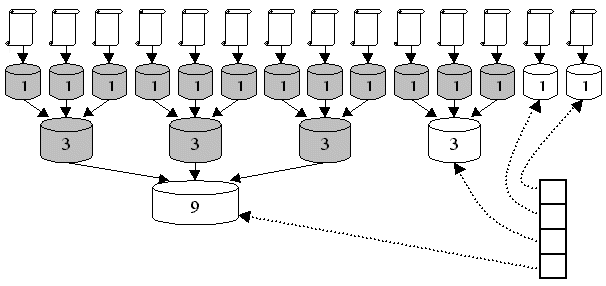
\includegraphics[width=0.8\textwidth]{indexing.png}
\caption{Lucene indexing}\label{fig:indexing}
\end{figure}

Such a merge techinque avoids frequent random modifications to inverted index file, because merge process itself could work in an disk-optimized way just like external sorting algorithm.
It reads records sequentially from all input index files, merge records in memory, and output results also in large sequential write. Hence it's not so slow even when inputs are too large to fit in physical memory.
So the technique can be adopted to solve our problem, merge sdb\_btree on disk from time to time so as to create huge sdb\_btree incrementally.

Let us describle it detailedly. There are two basic algorithms:
\begin{enumerate}
\item Keep an sdb\_btree in memory as cache, new records are always inserted into it. Save it as an on-disk sdb\_btree when cache gets full, after that clean the cache.
\item Merge on-disk sdb\_btree from time to time.
\end{enumerate}

In this way, we can eliminate all random writes, right? Because in algorithm 1 above, storing an in-memory sdb\_btree to disk is just to write several handred megabytes memory blocks to disk file for once.
And in algorithm 2 merge process only has large sequential reads and writes.

One short coming for this solution is, when in a state there are multiple unmerged sdb\_btree structures on disk, we have to search all of them to find value of an given key, hence speed for find operation is affected.
In order to applied for those ``insert-all-find-all-time'' applictions, an optimize() method is provided in hdb, which will force merge all sdb\_btree, both in-memory one and on-disk ones, together to be a single sdb.

\section{Modification tag}

Using merge-based incremental growth method, we can eliminate all random writes. But before inserting a new arrived record into in-memory sdb\_btree,
we still have to search those on-disk sdb\_btree structures, so as to find whether the key exists, which brings large numbers of random reads.
Now in this section, the task is to eliminate these random reads.

The premise to slove the problem is, don't try to find whether key exists and its location for new arrival record. The logic is easy to understand, if you search for its location or existance, random read is inevitable.

With this limitation in mind, I proposed a modification tag method. In which, each record is saved together with a tag indicating modification type to show how what operation is relevant with the record, e.g, insert, update or delete.
So each record in hdb looks like a triple: $<$key0, value0, INSERT$>$, $<$key1, value1, INSERT$>$, $\dots$ , $<$key0, $value0'$, UPDATE$>$, $<$key1, null, DELETE$>$.

I define four types of tag, INSERT, UPDATE, DELETE to support three basic operations, and an additional one called DELTA for applications that only want to increase orignal value in hdb by some $\Delta$.

\begin{itemize}
\item Insert

For new insertion, say, application developper calls insertValue function:
\begin{lstlisting}[language=C]
hdb.insertValue(key, value); 
\end{lstlisting}
Hdb just insert the record $<$key, value, INSERT$>$ into in-memory sdb\_btree when no record with the same key exists in in-memory sdb\_btree. If such a record exists and tag is INSERT or UPDATE or DELTA, do no modification,
or else if tag is DELETE, overwrite it.

\item Update

For update operations like:
\begin{lstlisting}[language=C]
hdb.updateValue(key, value); 
\end{lstlisting}
Hdb just insert the record $<$key, value, UPDATE$>$ into in-memory sdb\_btree when no record with the same key exists in in-memory sdb\_btree. If such a record exists always overwrite it.

\item Delete

\begin{lstlisting}[language=C]
hdb.delete(key); 
\end{lstlisting}
Hdb just insert the record $<$key, null, DELETE$>$ into in-memory sdb\_btree when no record with the same key exists in in-memory sdb\_btree. If such a record exists always overwrite it.

\item Delta

A most typical behavior in MIA's offline algorithm is, get the value for a given key, add 1 to the value, then update db.
\begin{lstlisting}[language=C]
ValueType tmp;
db.getValue(key, tmp);
tmp ++;
db.updateValue(key, tmp);
\end{lstlisting}
It seems to be a combination of find operation and update operation, which brings random reads. However, fundamentally, here developper doesn't care about exactly what the value is,
he just want to increase original value by some $\Delta$ (1 in above example).

So an additional interface called delta() is added to eliminate random reads here, ValueType should have ``+'' operator, and application developper write code in this way:
\begin{lstlisting}[language=C]
ValueType delta = 1;
db.delta(key, delta);
\end{lstlisting}
Hdb just insert the record $<$key, delta, DELTA$>$ into in-memory sdb\_btree when no record with the same key exists in in-memory sdb\_btree. If such a record exists,
\begin{enumerate}
\item if record is $<$key, value, INSERT$>$, overwrite it with $<$key, value+delta, INSERT$>$ if key doesn't exist in all on-disk sdb\_btree, or overwrite it with $<$key, delta, DELTA$>$.
\item if record is $<$key, value, UPDATE$>$, overwrite it with $<$key, value+delta, UPDATE$>$.
\item if record is $<$key, value, DELTA$>$, overwrite it with $<$key, value+delta, DELTA$>$.
\item if tag is DELETE, overwrite it by the record $<$key, 1, UPDATE$>$.
\end{enumerate}
So, it's encouraged to use update rather than insert together with delta, for hdb must search all sdb\_btree to see whether key exists so as to decide how to overwrite the record in in-memory sdb\_btree.

\end{itemize}

Just now we talked about how to implement four tyes of operations, they are all computations wholely in memory
(except in particular situation user calls insert before delta, but we recommend that, using together with delta, call update instead of insert).
As a result, records with the same key may exist between different sdb\_btree. So merging algorithm needs small modification to handle them, merging all records with the same key between different sdb\_btree.
Say there are N records with the same key found in different sdb\_btree, stored in an array Records, sorted by sdb\_btree's history, here is the code to merge their values:
\begin{lstlisting}[language=C]
ValueType accumulator;
for( i=0; i<N; i++)
{
  switch( Records[i].tag )
  {
  case INSERT:
  {
    if( accumulator is not set )
      accumulator = Records[i].value;
  }
  case UPDATE:
  {
    accumulator = Records[i].value;
  }
  case DELETE:
  {
    reset accumulator;
  }
  case DELTA:
  {
    accumulator += Records[i].value;
  }
}
\end{lstlisting}

Find values for a given key from serveral unmerged sdb\_btree is implemented in similar mannel. Search all records in separate btrees at first, then merge their values.

\section{Experiment}

Up to now, I have implemented an initial version of hdb, which supports insert method only. I compare random insertion performance with sdb\_btree, whose performance is given in section 1.

By setting merge factor to 4, 100,000,000 times random insertions can be finished within 13 minutes, while ocuppying less than 200M memory.

We can compare the result with sdb\_btree, which uses 1G memory, but still takes about one hour to insert 44,000,000 records. (so 100,000,000 times random insertions can be more than one day)

Experiment result shows, eliminating both random reads and random writes boost db's performance visibility for random insertions.

\section{Summary and conclusions}

In this draft, we check and analyse the reason why sdb\_btree has bad performance for random insertions, find it's due to inefficient random reads and writes.
Then we propose two techniques: merge-based incremental growth and modification tag to eliminate both of them, although at the cost of much slower find operation when hdb is in unmerged state
and store additional 1 byte tag field for each db record. Experiment shows the costs worth gains from efficient IO.

\section{Future work}

Sdb\_btree is just variants of classical banlanced multiway B\_tree in textbook, it isn't efficient enough to manage data on massive storage,
for example, it doesn't even adopt a B+\_tree structure currently. In B+\_tree, only leaf node contains data, and internal data have hundreds of child pointers,
thus more than 99\% pages are leaf pages, making it realistic that all or most internal node cached in memory at most of the time.
But in sdb\_btree, both internal nodes and leaf nodes contain data, the only difference is leaf nodes do not contain child pointers.
I believe find operations can be accerlated by using B+\_tree structure.

Besides, large number of materials has been published proposing various versions of B\_tree variants, such as write-optimized B\_tree, UB-trees and R-trees, understanding how they work and absorbing
their advantages into sdb\_btree would be of great benifit.

\end{document}